\documentclass[cn,chinese,color=cyan]{elegantbook}

\title{我的LaTeX课程}
\subtitle{入门学习笔记}
\author{雨霓同学}
\institute{910014191@qq.com}
\date{\today}
\bioinfo{QQ}{910014191}
\version{苓}

\extrainfo{别人都关心你飞的有多高,只有我关心你的翅膀好不好吃!}

\logo{233.png}
\cover{2 (12).jpg}

% 本文档命令
\usepackage{indentfirst}
\setmainfont{Times New Roman}
\usepackage{tcolorbox}
\tcbuselibrary{listings,breakable}
\tcbset{boxrule=0pt,sharp corners}
\renewcommand{\ttdefault}{cmtt}
\usepackage{tcolorbox}
\tcbuselibrary{breakable}
\tcbset{boxrule=0pt,sharp corners}
\renewcommand{\ttdefault}{cmtt}
\lstdefinestyle{mystyle}{
  basicstyle=%
    \ttfamily
    \lst@ifdisplaystyle\small\fi
}
\lstset{basicstyle=\ttfamily,style=mystyle}
\definecolor{lightgrey}{rgb}{0.9,0.9,0.9}
\definecolor{frenchplum}{RGB}{190,20,83}
\lstset{language=[LaTeX]TeX,
	texcsstyle=*\color{winered},
	numbers=none,
	breaklines=true,
	keywordstyle=\color{winered},
	commentstyle=\color{gray},
	emph={fontenc,fontspec,xeCJK,FiraMono,xunicode,newtxmath,figure,fig,image,img,table,itemize,enumerate,newtxtext,newtxtt,ctex,microtype,description,times,newtx,booktabs,tabular,PDFLaTeX,XeLaTeX,type1cm,BibTeX,device,color,mode,lang,amsthm,tcolorbox,titlestyle,cite,marginnote,ctex,listings},
	emphstyle={\color{frenchplum}},
	morekeywords={DeclareSymbolFont,SetSymbolFont,toprule,midrule,bottomrule,institute,version,includegraphics,setmainfont,setsansfont,setmonofont ,setCJKmainfont,setCJKsansfont,setCJKmonofont,RequirePackage,figref,tabref,email,maketitle,keywords,definecolor,extrainfo,logo,cover,subtitle,appendix,chapter,hypersetup,mainmatter,tableofcontents,elegantpar,numbers,authoryear,heiti,kaishu,lstset,pagecolor,zhnumber,marginpar,part,equote},
	frame=single,
	tabsize=2,
	rulecolor=\color{structurecolor},
	framerule=0pt,
	columns=flexible,
	% backgroundcolor=\color{lightgrey}
}
\lstdefinestyle{R}{	
	language={[LaTeX]TeX},
	numbers=left,
	numbersep=1em,
	numberstyle=\tiny,
	frame=single,
	framesep=\fboxsep,
	framerule=\fboxrule,
	rulecolor=\color[RGB]{31, 186, 190},
	xleftmargin=\dimexpr\fboxsep+\fboxrule\relax,
	xrightmargin=\dimexpr\fboxsep+\fboxrule\relax,
	breaklines=true,
	basicstyle=\small\tt,
	keywordstyle=\color{blue},
	commentstyle=\color[RGB]{33, 33, 33},
	backgroundcolor=\color[RGB]{233, 248, 248},
	tabsize=2,
	columns=flexible,
	morekeywords={maketitle},
}
\numberwithin{equation}{section}
\usepackage{cases,empheq}
\usepackage{booktabs}  % 绘制三线表的线
\usepackage{tikz} 
\usepackage{array}
\usepackage{float}
\usepackage{halloweenmath}
\usepackage{longtable}
\usepackage{tabularx}
\usepackage{pifont}
\usepackage{enumitem}
\usepackage{subfig}

\newcommand{\ccr}[1]{\makecell{{\color{#1}\rule{1cm}{1cm}}}}
% 修改目录深度
\setcounter{tocdepth}{2}

% 修改目录深度
\setcounter{tocdepth}{2}

\begin{document}
\frontmatter
\definecolor{mycolor}{RGB}{198, 182, 200}%用于设置封面长条颜色
\maketitle
\tableofcontents
\mainmatter	
\chapter*{特别声明}
\markboth{Introduction}{前言}
在此特别感谢,\href{https://elegantlatex.org/}{Elegant\LaTeX{}} 系列模板的各位作者大大,没有他们我去哪里找这么好看的模板。这是模板的一些地址:\href{https://github.com/ElegantLaTeX}{GitHub}、\href{https://ctan.org/pkg/elegantbook}{CTAN}、\href{https://www.overleaf.com/latex/templates/elegantbook-template/zpsrbmdsxrgy}{Overleaf} 以及 \href{https://gitee.com/ElegantLaTeX/ElegantBook}{Gitee}感兴趣的同学的可以自己下载! 

关于为什么有这个内容的存在?emmmm卤煮大概是大三的时候学习的\LaTeX 。平时主要用这个排版一些学习笔记,后来大大小小的学术期刊、论文都排过一些,所以慢慢就想着把自己学习\LaTeX 的内容记录一下,于是就有了这个玩意!希望能够帮助到想要学习或者入门\LaTeX 的同学!



\underline{如果你发现我写的内容,那些地方有问题,希望可以留言给我},联系方式在封面页!这里会尽可能的改正!目前还有一些Bug没能解决,希望有能力的大佬帮助解决下!(第一处笔记处有记录)

\vskip 1.5cm

\begin{flushright}
	梁霄\\
	\today
\end{flushright}
	
	

\chapter{LaTeX 入门之公式篇}
\begin{introduction}
	\item 数学模式
	\item 常用数学宏包
	\item 公式的编号
	\item 公式环境
	\item 定界符宏包
	\item 矩阵环境
\end{introduction}
\section{数学模式}
\subsection{行内公式}
LaTeX提供三种方法来编写行内公式
\begin{enumerate}
	\item \verb|$...这是公式内容...$|
	\item  \verb|\(...这是公式内容...\)|
	\item  \verb|\begin{math}...这是公式内容...\end{math}|
\end{enumerate}
如有如下示例:
\begin{tcblisting}{sidebyside}
四叶线玫瑰线 $p=a\sin2\beta$方程 

四叶线玫瑰线\(p=a\sin2\beta\)方程 

四叶线玫瑰线
\begin{math}p=a\sin2\beta\end{math}方程
\end{tcblisting}
\begin{note}
	常用的行内数学模式效果是一样的,不过第一种方法是比较常用的,原因嘛,使用方便,但是缺点是不能区分起止,还有一种原因是因为它性格坚强(是因为它能出现在一些其他命令中,像上面的\verb+\verb|text|+这就是一个脆弱命令,它不能直接出现在任何命令中。(\$这个符号的公式显示貌似有点bug,代码区域不显示\$符号)
\end{note}

\subsection{行间公式}
LaTeX提供三种方法来编写行内公式
\begin{enumerate}
\item \verb|$$...这是公式内容...$$|
\item  \verb|\[...这是公式内容...\]|
\item  \verb|\begin{displaymath}...这是公式内容...\end{displaymath}|
\end{enumerate}
如有如下示例:
\begin{tcblisting}{sidebyside}
四叶线玫瑰线:$$p=a\sin2\beta$$方程.

四叶线玫瑰线:\[p=a\sin2\beta\]方程. 

四叶线玫瑰线:
\begin{displaymath}
p=a\sin2\beta
\end{displaymath}
方程.
\end{tcblisting}
\begin{note}
	常用的行内数学模式效果是一样的,也是第一种方法是比较常用,这是\TeX 的原始方法,只有在极个别的情况下会出现问题(fleqn)环境中,在数学模式中一般不建议出现空行或者\verb|\par|等换行命令,因为系统会提示出错。
\end{note}
\section{常用数学宏包}
\subsection{花式数学字体}
常见公式宏包\verb|amsmath、mathrsfs、amsfonts、bm|宏包导言区使用\verb|\usepackage{amsmath}|

\begin{tcblisting}{sidebyside}
$$\mathscr{ABCDEFGHI}$$
$$\mathcal{ABCDEFGHI}$$
$$\mathbb{ABCDEFGHI}$$
$$\mathfrak{ABXDEFGHI}$$
\end{tcblisting}

\subsection{公式字体加粗}
\begin{tcblisting}{sidebyside}
$$\bm{X^2+Y^2=Z^2}$$
$$\mathbf{{X^2+Y^2=Z^2}}$$
$${X^2+Y^2=Z^2}$$
\end{tcblisting}
这一部分通常不太用,看需求吧,如果你有花里胡哨的需求,可以参考symbols-a4.pdf这本书,里面各种花里胡哨的符号都有,很强大,书籍地址:\href{https://pan.baidu.com/s/1mBsAbj6PrPY5GycyU1V1FQ}{提取码:cycb点击跳转}
\newpage
\section{公式的编号}
\subsection{公式的自动编号}
一般情况都是行间公式才会进行公式编号,那么如何进行编号呢?
\begin{tcblisting}{sidebyside}
这是一个行间公式,我们可以使用
\begin{equation}
\lim _{x \rightarrow 0}\int_{0}^{x} \frac{t^{2}}{\sqrt{a+t^{2}}} d t=1
\end{equation}
进行行间公式编号
\end{tcblisting}
\subsection{使用标签自定义编号}
当然也可以使用一些标签进行自定义编号,一般很少这样子用,示例如下:
\begin{tcblisting}{sidebyside}
这是一个行间公式,我们可以使用\verb|\tag{*}|
\begin{equation}\tag{*}
\lim _{x \rightarrow 0}\int_{0}^{x} \frac{t^{2}}{\sqrt{a+t^{2}}} d t=1
\end{equation}
进行行间公式标签自定义编号
\end{tcblisting}
\subsection{公式的重新编号}
我们可以使用自定义命令,让原本按章编号的公式现在按节进行编号,这个准确的名称叫做公式的排序单位
\begin{tcblisting}{sidebyside}
\numberwithin{equation}{section}
这是按节编号
\begin{equation}
\lim _{x \rightarrow 0}\int_{0}^{x} \frac{t^{2}}{\sqrt{a+t^{2}}} d t=1
\end{equation}
进行行间公式编号
\end{tcblisting}

\begin{tcblisting}{sidebyside}
\numberwithin{equation}{chapter}
这里是按章进行编号,注意看
\begin{equation}
\lim _{x \rightarrow 0}\int_{0}^{x} \frac{t^{2}}{\sqrt{a+t^{2}}} d t=1
\end{equation}
\end{tcblisting}
\begin{note}
我们可以通过更改\verb|\numberwithin{equation}{section}|中的section选项来改变编号形式,这里默认是section。
\end{note}
\subsection{公式的子编号}
有时候一个行间公式有多个子公式,这时候需要对每个子公式进行编号,可以这样子去做。
\numberwithin{equation}{section}
\begin{tcblisting}{sidebyside}
这是多公式进行子编号
\begin{subequations}
\begin{equation}\
\lim _{x \rightarrow 0} \frac{1}{b x-\sin x}dx
\end{equation}
\begin{equation}
\lim _{x \rightarrow 0} \frac{1}{b x-\sin x}dx
\end{equation}
\end{subequations}
\end{tcblisting}
同样的我们也可以使用标签进行自定义命令,
\begin{tcblisting}{sidebyside}
\begin{subequations}
\begin{equation}\tag{$\alpha$}
\underset{x\to 0}{\mathop{\lim }}\,\int_{0}^{x}
{\frac{{{t}^{2}}}{\sqrt{a+{{t}^{2}}}}dt=1}
\end{equation}
\begin{equation}\tag{$\beta$}
\underset{x\to 0}{\mathop{\lim }}\,\int_{0}^{x}
{\frac{{{t}^{2}}}{\sqrt{a+{{t}^{2}}}}dt=1}
\end{equation}
\end{subequations}
\end{tcblisting}

同样的也可以使用汉字进行编号
\begin{tcblisting}{sidebyside}
\begin{subequations}
\begin{equation}\tag{$\text{公式1}$}
\lim _{x \rightarrow 0} \frac{1}{b x-\sin x}dx
\end{equation}
\begin{equation}\tag{$\text{公式2}$}
\lim _{x \rightarrow 0} \frac{1}{b x-\sin x}dx
\end{equation}
\end{subequations}
\end{tcblisting}
\subsection{其他补充编号}
还有一些其他的编号方式,这里做下整理,也可以参照示例:
\begin{table}[H]
	\centering
	\begin{tabular}{m{3cm}m{10cm}}
		\toprule
		\verb|\eqno{标号}| &系统提供的一个序号设置命令,可以放在equation*或\verb|\[...\]|形式的公式行后,可以在公式右侧人工设置编号,标号是任意文本 \\
		\verb|leqno{标号}|
		&作用与\verb|\eqno{标号}|相似,只是将标号置于公式的左侧。对了两个不能同时使用,也不会出现这样奇葩的需求吧!\\
		\verb|\nonumber|
		&系统提供的取消序号命令,可以把它插在换行命令之前,就可以为取消改行公式的序号\\
		\verb|\notag|
		& 和nonumber是一样的\\
		\verb|\tag*{标号}|
		&和\verb|\tag{label}|相同,只是标号两侧没有圆括号\\
		\bottomrule
	\end{tabular}
\end{table}
\begin{tcblisting}{sidebyside}
使用\verb|\eqno{标号}|
\begin{equation*}
\lim _{x \rightarrow 0}\int_{0}^{x} \frac{t^{2}}{\sqrt{a+t^{2}}} d t=1\eqno{\text{公式1}}
\end{equation*}
\end{tcblisting}
\begin{tcblisting}{sidebyside}
使用\verb|\leqno{标号}|
\begin{equation*}
\lim _{x \rightarrow 0}\int_{0}^{x} \frac{t^{2}}{\sqrt{a+t^{2}}} d t=1\leqno{\text{公式1}}
\end{equation*}
\end{tcblisting}

\begin{tcblisting}{sidebyside}
使用\verb|\nonumber|
\begin{align}
(a+b)^{4} &=(a+b)^{2}(a+b)^{2} \\ 
&=\left(a^{2}+2 a b+b^{2}\right)\left(a^{2}+2 a b+b^{2}\right) \nonumber \\ 
&=a^{4}+4 a^{3} b+6 a^{2} b^{2}+4 a b^{3}+b^{4} \nonumber
\end{align}
\end{tcblisting}

\begin{tcblisting}{sidebyside}
使用\verb|\notag|
\begin{align}
(a+b)^{4} &=(a+b)^{2}(a+b)^{2} \\ 
&=\left(a^{2}+2 a b+b^{2}\right)\left(a^{2}+2 a b+b^{2}\right) \notag \\ 
&=a^{4}+4 a^{3} b+6 a^{2} b^{2}+4 a b^{3}+b^{4} \notag
\end{align}
\end{tcblisting}
\begin{tcblisting}{sidebyside}
使用\verb|\tag*{标号}|
\begin{equation}
\lim _{x \rightarrow 0}\int_{0}^{x} \frac{t^{2}}{\sqrt{a+t^{2}}} d t=1\tag*{\text{公式1}}
\end{equation}
\end{tcblisting}
\begin{tcblisting}{sidebyside}
使用\verb|\tag{标号}|
\begin{equation}
\lim _{x \rightarrow 0}\int_{0}^{x} \frac{t^{2}}{\sqrt{a+t^{2}}} d t=1\tag{\text{公式1}}
\end{equation}
\end{tcblisting}
\newpage
\section{amsmath的公式环境}
公式宏包amsmath是由美国数学学会组织编写的一个公式宏包,它是ams宏包套件众最主要的宏包,现在编写行间公式通常采用amsmath提供的各种公式环境。具体如下表所示:
\begin{table}[H]
	\centering
	\caption{公式宏包amsmath提供的各种公式环境}
	\begin{tabular}{m{2cm}m{4cm}m{2cm}m{4cm}}
		\toprule
		环境名&用途&环境名&用途 \\  \midrule
		equation &	单行公式环境 &equation*&单行公式环境,无序号\\
		align & 公式组环境 &align* & 公式组环境,无序号 \\
		alignat & 公式组环境 &alignat* & 公式组环境,无序号 \\
		flalign & 公式组环境 &flalign* & 公式组环境,无序号 \\
		gather & 公式组环境 &gather* & 公式组环境,无序号 \\ \midrule
		aligned & 块环境,无序号 &alignedat& 块环境,无序号 \\
		gathered &块环境,无序号,&~&\\ \midrule
		multline & 多行公式环境 &multline*&多行公式环境,无序号 \\
		split & 多行公式环境,无序号 &~&~\\
		cases &左花括号环境,无序号 &subequations &子公式环境 \\
		\bottomrule		
	\end{tabular}
\end{table}
具体示例如下:
\subsection{equation环境}
单行公式环境equation无论公式多长,都可以排为一行,并给出一个序号,使用equation*则可以去掉序号。
\begin{tcblisting}{sidebyside}
单行公式环境equation
\begin{equation}
f(x)=3x^2+6(x-2)-1
\end{equation}
\vskip 2mm \hrule \vskip 2mm
单行公式环境equation*
\begin{equation*}
f(x)=3x^2+6(x-2)-1
\end{equation*}
\end{tcblisting}

\subsection{align,align*,aligned环境}
如果要求共十组或多行公式以其中某个符号对齐,可以align环境环境,它以\verb|\\|为分行符,每行都输出序号,它以\verb|&|为分列标志,奇数列右对齐,偶数列左对齐,奇偶列并肩对齐
\begin{tcblisting}{sidebyside}
这是align环境
\begin{align} 
f(x) &=2(x+1)^{2}-1 \\
&=2 x^{2}+4 x+1 
\end{align}
\end{tcblisting}
\begin{tcblisting}{sidebyside}
这是align*环境,不需要数学模式
\begin{align*} 
f(x) &=2(x+1)^{2}-1 \\
&=2\left(x^{2}+2 x+1\right)-1 \\ 
&=2 x^{2}+4 x+1 
\end{align*}
\end{tcblisting}
\begin{tcblisting}{sidebyside}
aligned环境需要数学模式
$$\begin{aligned} 
f(x) &=2(x+1)^{2}-1 \\
&=2\left(x^{2}+2 x+1\right)-1 \\ 
&=2 x^{2}+4 x+1 
\end{aligned}$$
\end{tcblisting}
\subsection{alignat,alignat*,alignedat环境}
公式组alignat环境与align环境相似,不同之处在于列对之间的默认距离为0pt,通常要插入水平空白命令,用于控制列对之间的距离,此外该环境还有一个参数项,用于设置列的个数,其数目需大于实际值,但不能小于。
\begin{tcblisting}{sidebyside}
alignat环境不需要数学模式
\begin{alignat}{3}
A_{1}&=B_{1} B_{2} \quad &A_{3}&=B_{1} \\ 
A_{2}&=B_{3} & A_{3} A_{4}&=B_{4}
\end{alignat}
\end{tcblisting}
\begin{tcblisting}{sidebyside}
alignat环境不需要数学模式
\begin{alignat*}{3}
A_{1}&=B_{1} B_{2} \quad &A_{3}&=B_{1} \\ 
A_{2}&=B_{3} & A_{3} A_{4}&=B_{4}
\end{alignat*}
\end{tcblisting}
\begin{tcblisting}{sidebyside}
alignatedat环境需要数学模式
$$\begin{alignedat}{3}
A_{1}&=B_{1} B_{2} \quad &A_{3}&=B_{1} \\ 
A_{2}&=B_{3} & A_{3} A_{4}&=B_{4}
\end{alignedat}$$
\end{tcblisting}
\subsection{gather,gather*,gathered环境}
gather用于编写中心对称的公式组,使用换行命令来区分各个命令,每个公式都与公式行居中对齐。

\begin{tcblisting}{sidebyside}
gather环境不需要数学模式
\begin{gather}
\ln y=x \ln x \\
y^{\prime}=x^{x}(1+\ln x)
\end{gather}
\end{tcblisting}
\begin{tcblisting}{sidebyside}
gather*环境不需要数学模式
\begin{gather*}
\ln y=x \ln x \\
y^{\prime}=x^{x}(1+\ln x)
\end{gather*}
\end{tcblisting}
\begin{tcblisting}{sidebyside}
gathered环境需要数学模式
$$\begin{gathered}
\ln y=x \ln x \\
y^{\prime}=x^{x}(1+\ln x)
\end{gathered}$$
\end{tcblisting}
\subsection{flalign,multline}
falign与align的功能基本相同,唯一区别是列对之间的距离为弹性宽度,以使公式组两端对齐
\begin{tcblisting}{sidebyside}
flalign环境不需要数学模式
\begin{flalign}{3}
A_{1}&=B_{1} B_{2}  &A_{3}&=B_{1} \\ 
A_{2}&=B_{3} & A_{3} A_{4}&=B_{4}
\end{flalign}
\end{tcblisting}
\begin{tcblisting}{sidebyside}
flalign环境不需要数学模式
\begin{flalign*}{3}
A_{1}&=B_{1} B_{2}  &A_{3}&=B_{1} \\ 
A_{2}&=B_{3} & A_{3} A_{4}&=B_{4}
\end{flalign*}
\end{tcblisting}
多行公式环境multlins可用于编写多行公式,首航左对齐,尾行右对齐,中间居中对齐,公式编号在行尾给出。
\begin{tcblisting}{sidebyside}
multline环境不需要数学模式
\begin{multline} A_{m}^{n}=m(m-1) \\
+(m-2) 
\\+[m-(n-1)] 
\end{multline}
\end{tcblisting}
\begin{tcblisting}{sidebyside}
\begin{multline*} A_{m}^{n}=m(m-1) \\
+(m-2) 
\\+[m-(n-1)] 
\end{multline*}
\end{tcblisting}
使用\verb|\shoveleft,\shoveright|可以使中间公式左对齐或者右对齐
\begin{tcblisting}{sidebyside}
\begin{multline} A_{m}^{n}=m(m-1) \\
\shoveleft{+(m-2)} \\
+[m-(n-1)] 
\end{multline}
\begin{multline*} A_{m}^{n}=m(m-1) \\
\shoveright{+(m-2)} \\
+[m-(n-1)] 
\end{multline*}
\end{tcblisting}
\begin{note}
	这个总感觉不太好用
\end{note}
\subsection{split环境}
split也用于排版多行公式,它与multline的区别主要是以下三点。
\begin{enumerate}
\item 使用\verb|&|作为分隔符,但至多两列,左列右对齐,右列左对齐,如果不使用分隔符,则所有公式行为一列,且全部与首航公式右端对齐
	\item 必须置身于除multline环境之外的其他公式环境中
	\item 自身并不生成公式序号,而是由外在公式环境提供,序号垂直居中 
\end{enumerate}

\begin{tcblisting}{sidebyside}
\begin{equation}
\begin{split} 
f(x) &=2(x+1)^{2}-1 \\
&=2\left(x^{2}+2 x+1\right)-1 \\ 
&=2 x^{2}+4 x+1 \end{split}
\end{equation}
\end{tcblisting}
\subsection{array,eqnarray环境}
数组宏包array对系统提供的数组环境array做了功能扩展,其参数位置和列格式的各种选项及功能与表格环境完全相同

\begin{tcblisting}{sidebyside}
\begin{equation*}
\left. \begin{array}{>{\kaishu} r ccl}
\text{常数}) &y&=&c \\
\text{直线}) &y&=&cx+d \\
\text{抛物线}) &y&=&bx^2+cx+d \\
\end{array}\right\} \text{多项式}
\end{equation*}
\end{tcblisting}
eqnarray公式组环境是由系统提供的,其默认公式对齐方式为右对齐。
\begin{tcblisting}{sidebyside}
\begin{eqnarray}
E = \hbar \cdot\nu \\
E = m \cdot c^2
\end{eqnarray}
\end{tcblisting}
\begin{tcblisting}{sidebyside}
\begin{eqnarray}
E &=& \hbar \cdot\nu \\
E &=& m \cdot c^2
\end{eqnarray}
\end{tcblisting}
\subsection{单花括号环境}
\subsubsection{左花括号环境}
左花括号环境cases用于在其他公式环境中排版带有左花括号的公式
\begin{tcblisting}{sidebyside}
\begin{equation}
|x| = 
\begin{cases}
x& \text{如果$x \geqslant 0$} \\
-x& \text{如果$x \leqslant 0$} \\
\end{cases}
\end{equation}
\end{tcblisting}
\begin{tcblisting}{sidebyside}
\begin{subnumcases}{|x| = }
x& $x \geqslant 0$ \\
-x& $\leqslant 0$
\end{subnumcases}
\end{tcblisting}
\begin{tcblisting}{sidebyside}
\begin{numcases}{|x| = }
x& $x \geqslant 0$ \\
-x& $\leqslant 0$
\end{numcases}
\end{tcblisting}
\subsubsection{右花括号环境}
右花括号环境rcases用于在其他公式环境中排版带有左花括号的公式
\begin{tcblisting}{sidebyside}
\begin{equation*}
\begin{rcases}
\text{正无理数} \\
\text{负无理数}
\end{rcases}
\text{无限不循环小数}
\end{equation*}
\end{tcblisting}
\section{定界符宏包}
给带定界符的方程组的每一行都编号,这种情况\textbf{amsmath}包无法实现,我们可以用\textbf{cases}包的\textbf{numcases}环境
\begin{tcblisting}{sidebyside}
%\usepackage{cases}
\begin{numcases}{f(x)=}%f(x)=可以置空
1,&$x\in\mathbb Q$\\
0,&$x\notin\mathbb Q$
\end{numcases}.
\end{tcblisting}
不过上述\textbf{numcases}环境的效果是不尽如人意的,更好的效果是用\textbf{empheq}包,它可以给\textbf{amsmath}包提供的数学环境添加各种定界符.
\begin{tcblisting}{sidebyside}
\begin{empheq}[left=\empheqlbrace,
right=\empheqrbrack]{align}
&a=b+c&&a=b\\
&a^2=b^2+c^2&&a=b
\end{empheq}
\end{tcblisting}

\section{矩阵环境}
常用的矩阵输入,可以使用array、matrix、Bmatrix、bmatrix、Pmatrix、vmatrix、Vmatrix等等
\subsection{array 环境}
需要使用数学模式
\begin{tcblisting}{sidebyside}
$$\left[
\begin{array}{ccc}
1&2&3 \\4&5&6 \\7&8&9 \\
\end{array}
\right]$$
\end{tcblisting}

\begin{tcblisting}{sidebyside}
$$
\left\{
\begin{array}{ccc}
1&2&3 \\
4&5&6 \\
7&8&9 \\
\end{array}
\right\}
$$
\end{tcblisting}

\begin{tcblisting}{sidebyside}
$$
\left|
\begin{array}{ccc}
1&2&3 \\
4&5&6 \\
7&8&9 \\
\end{array}
\right|
$$
\end{tcblisting}


\begin{tcblisting}{sidebyside}
$$
\left(
\begin{array}{ccc}
1&2&3 \\
4&5&6 \\
7&8&9 \\
\end{array}
\right)
$$
\end{tcblisting}
\subsection{matrix 环境}
需要使用数学模式
\begin{tcblisting}{sidebyside}
$$
\begin{matrix}
1&2&3 \\
4&5&6 \\
7&8&9 \\
\end{matrix}
$$
\end{tcblisting}


\begin{tcblisting}{sidebyside}
\[
\left[
\begin{matrix}
1&2&3 \\
4&5&6 \\
7&8&9 \\
\end{matrix}
\right]
\]
\end{tcblisting}

\subsection{bmatrix 环境}
\begin{tcblisting}{sidebyside}
\[
\begin{bmatrix}
1&2&3 \\
4&5&6 \\
7&8&9 \\
\end{bmatrix}
\]
\end{tcblisting}


\subsection{Bmatrix 环境}
\begin{tcblisting}{sidebyside}
$$
\begin{Bmatrix}
1&2&3 \\
4&5&6 \\
7&8&9 \\
\end{Bmatrix}
$$
\end{tcblisting}
\subsection{pmatrix 环境}
\begin{tcblisting}{sidebyside}
\begin{equation}\tag{***}
\begin{pmatrix}
1&2&3 \\
4&5&6 \\
7&8&9 \\
\end{pmatrix}\label{ces}
\end{equation}
\end{tcblisting}



\subsection{vmatrix 环境}
\begin{tcblisting}{sidebyside}
\begin{equation}\tag{***}
\begin{vmatrix}
1&2&3 \\
4&5&6 \\
7&8&9 \\
\end{vmatrix}\label{ces}
\end{equation}
\end{tcblisting}

\subsection{Vmatrix 环境}
\begin{tcblisting}{sidebyside}
$$
\begin{Vmatrix}
1&2&3 \\
4&5&6 \\
7&8&9 \\
\end{Vmatrix}
\leqno{(\text{公式1})}$$
这是公式\ref{ces}
\end{tcblisting}



\begin{tcblisting}{sidebyside}
\[
\left[\begin{array}{cccc}
w_{11}& w_{12}& \cdots& w_{1 n} \\
w_{21}& w_{22}&\ldots& w_{2 n}\\
{\cdot}& ~ & ~ & ~\\
{\cdot} &~ &~ & ~\\
w_{n 1} &w_{n 2}& \ldots& w_{n n}
\end{array} \right]
\]
\end{tcblisting}




\chapter{LaTeX 入门之表格篇}
\begin{introduction}
	\item 常用表格环境
	\item 跨行表格
	\item 表格浮动
	\item 三线表跨页表
	\item 其他表格宏包
	\item 列表的使用
\end{introduction}
\section{常用表格环境tabular}
\LaTeX 里排版表格不如Word 等所见即所得的工具简便和自由,不过对于不太复杂的表格来讲,完全能够胜任。

数组宏包array改进了扩展了\LaTeX 的tabular,tabular*和arraya的功能环境,主要是增强了列格式功能,还添加了许多表格参数的功能调整,array和tabular环境相似。

排版表格最基本的tabular环境用法为:
\begin{lstlisting}[style=R]
\begin{tabular}[<垂直对齐方式>]{<列格式说明>}
<单元格内容> & ... & <单元格内容> \\
.....
<单元格内容> & ... & <单元格内容> \\
\end{tabular}
\end{lstlisting}
\subsection{垂直对齐方式设置}
\begin{itemize}
	\item t:表格顶线与当前文本行的基线对齐
	\item c: 默认参数,表格中线与当前文本行的基线对齐
	\item b: 表格底线与当前文本行的基线对齐
	\item \verb|\fisthline| : 更改t参数的对齐方式
	\item \verb|\lasthline| :更改b参数的对齐方式
\end{itemize}


\begin{tcblisting}{sidebyside}
这是文本行:
\begin{tabular}[c]{|l|l|} \hline
<1> & <2> \\ \hline
<3> & <4>  \\ \hline
\end{tabular}
\vskip 3mm
这是文本行:
\begin{tabular}[t]{|l|l|} \hline
<1> & <2> \\ \hline
<3> & <4>  \\ \hline
\end{tabular}
\end{tcblisting}
\begin{tcblisting}{sidebyside}
这是文本行:
\begin{tabular}[b]{|l|l|} \hline
<1> & <2> \\ \hline
<3> & <4>  \\ \hline
\end{tabular}
\vskip 3mm
这是文本行:
\begin{tabular}[b]{|l|l|} \hline
<1> & <2>  \\ \hline
<3> & <4> \\ \lasthline
\end{tabular}
\vskip 3mm
这是文本行:
\begin{tabular}[t]{|l|l|} \firsthline
<1> & <2>  \\ \hline
<3> & <4> \\ \hline
\end{tabular}
\end{tcblisting}

\subsection{列格式说明}
\begin{itemize}
	\item l:左对齐
	\item c: 居中对齐
	\item r: 右对齐
	\item |:画纵向的线
\end{itemize}
\begin{tcblisting}{sidebyside}
1.左对齐\par
\begin{tabular}{|l|l|l|}\hline
\bfseries left &\bfseries center &\bfseries right\\ \hline
左对齐&居中对齐&右对齐\\ \hline
\end{tabular}\par
2.居中对齐\par
\begin{tabular}{|c|l|l|}\hline
\bfseries left &\bfseries center &\bfseries right\\ \hline
左对齐&居中对齐&右对齐\\ \hline
\end{tabular}\par
3.1.居中对齐\par
\begin{tabular}{|r|r|r|}\hline %{*{3}{|r}|}
\bfseries left &\bfseries center &\bfseries right\\ \hline
左对齐&居中对齐&右对齐\\ \hline
\end{tabular}
\end{tcblisting}
\subsection{其他参数}
\begin{description}
	\item[1. *\{n\}\{列格式\} ] 表示$n$个列格式选项相同的相邻列,例如\verb+*{3}{|c}|+,它表示表格中相邻三列的列格式是相同的;每列数据居中排列并且两侧都有一条垂直线,它等效于列格式:\verb+|c|c|c|+.
	\item[2. $p$\{宽度\}] 设定该列所占的宽度,并且该列数据左对齐排列,垂直方向顶端对齐。
	\item[3. $m$\{宽度\}] 设定该列所占的宽度,并且列数据左对齐排列,垂直方向中心对齐
	\item[4. $b$\{宽度\}] 设定该列所占的宽度,并且该列数据左对齐排列,垂直方向底端对齐
\end{description}

示例如下:
\begin{lstlisting}[style=R]
$p$\{宽度\}

\begin{tabular}{|p{3cm}|p{3cm}|p{5cm}|} \hline
<单元格> & <单元格内容单元格内>& <单元格> \\ \hline
<单元格> & <单元格内容><单元格内容> & <单元格> \\ \hline
\end{tabular}
	
$m$\{宽度\}

\begin{tabular}{|m{3cm}|m{3cm}|m{5cm}|}  \hline
<单元格> & <单元格内容单元格内>& <单元格> \\ \hline
<单元格> & <单元格内容><单元格内容> & <单元格> \\ \hline
\end{tabular}

$b$\{宽度\}

\begin{tabular}{|b{3cm}|b{3cm}|b{5cm}|}  \hline
<单元格> & <单元格内容单元格内>& <单元格> \\ \hline
<单元格> & <单元格内容><单元格内容> & <单元格> \\ \hline
\end{tabular}
\end{lstlisting}

\begin{enumerate}
	\item $p$\{宽度\}
	\vskip 2mm 
	\begin{tabular}{|p{3cm}|p{3cm}|p{5cm}|} \hline
		<单元格> & <单元格内容单元格内>& <单元格> \\ \hline
		<单元格> & <单元格内容><单元格内容> & <单元格> \\ \hline
	\end{tabular}
	\vskip 2mm 	
	\item $m$\{宽度\}
	\vskip 2mm 
	\begin{tabular}{|m{3cm}|m{3cm}|m{5cm}|}  \hline
		<单元格> & <单元格内容单元格内>& <单元格> \\ \hline
		<单元格> & <单元格内容><单元格内容> & <单元格> \\ \hline
	\end{tabular}
	\vskip 2mm 
	\item $b$\{宽度\}
	\vskip 2mm 
	\begin{tabular}{|b{3cm}|b{3cm}|b{5cm}|}  \hline
		<单元格> & <单元格内容单元格内>& <单元格> \\ \hline
		<单元格> & <单元格内容><单元格内容> & <单元格> \\ \hline
	\end{tabular}
\end{enumerate}
\begin{note}
	\verb|\hline|:该命令必须用于首行之前或者紧跟在换行命令\verb|\\|之后,它表示画一条长度与表格宽度相同的水平线,数据之间的分列符用\verb|&|表示
	
	\verb|\cline{i-j}|表示从$i$列的左侧到第$j$列起画一条水平线
\end{note}













\section{跨行表格宏包multirow}
\LaTeX 是一行一行排版表格的,横向合并单元格较为容易,由 \verb|\multicolumn| 命令实现:
\begin{lstlisting}[style=R]
\multicolumn{⟨n⟩}{⟨column-spec⟩}{⟨item⟩}
\end{lstlisting}
其中$ ⟨n⟩$ 为要合并的列数,$⟨column-spec⟩$ 为合并单
元格后的列格式,只允许出现一个$ l/c/r $或$p $格式。如果合并前的单元格前后带表格线 |,合并后的列格式也要带 | 以使得表格的竖线一致.item则是表格的内容。
\begin{tcblisting}{sidebyside}
\begin{tabular}{|c|c|c|}
\hline
1 & 2 & Center \\ \hline
\multicolumn{2}{|c|}{3} &
\multicolumn{1}{r|}{Right} \\ \hline
4 & \multicolumn{2}{c|}{C} \\ \hline
\end{tabular}
\end{tcblisting}
\begin{note}
	该命令可以用来修改某一个单元格的列格式。\verb|\multicolumn{1}{⟨column-spec⟩}{⟨item⟩}|
\end{note}

纵向合并单元格需要用到multirow宏包提供的\verb|\multirow| 命令:
\begin{lstlisting}[style=R]
\multirow{所跨行数}{数据宽度}{数据}
\end{lstlisting}
\begin{tcblisting}{sidebyside}
\begin{tabular}{|c|c|}
\hline
\multirow{4}{*}{相亲数}
& 220 \\ \cline{2-2}
& 284 \\ \cline{2-2}
&1210 \\ \cline{2-2}
&1184 \\ \hline 
\end{tabular}
\end{tcblisting}
我们看一个结合\verb|\cline、\multicolumn |和\verb|\multirow| 命令的例子:
\begin{tcblisting}{sidebyside}
\begin{tabular}{ccc}
\hline
\multirow{2}{*}{Item} &
\multicolumn{2}{c}{Value} \\
\cline{2-3}
& First & Second \\ \hline
A & 1 & 2 \\ \hline
\end{tabular}
\end{tcblisting}

\section{表格的浮动环境}
控制表格在本页显示位置需要table 环境,参数有htbp 四种,分别表示here,top,bottom,page of float.

table 环境中可以通过\verb|\caption| 命令为表格添加标题.

\subsection{位置参数}
\begin{enumerate}
	\item $h$ :指定将该浮动体就地放置,即放置在该浮动环境所在的位置,如果版面所剩空间放不下该浮动体,作者又没有指定其他选项,系统则将h改为t,即尝试将该浮动体放置到下一页的顶部
	
	\item $t$ 表示将该浮动体放置到当前页或下一页的顶部
	
	\item $b$ 表示将该浮动体放置到当前页或下一页的底部
	
	\item $p$ 表示将该浮动体放置在当前页之后的单独一页,该页被称为浮动体页page of float.
\end{enumerate}
该命令的使用方法如下:
\begin{lstlisting}[style=R]
\begin{table}[位置参数]
\caption{表格标题}
\begin{tabular}[<垂直对齐方式>]{<列格式说明>}
<单元格内容> & ... & <单元格内容> \\
.....
<单元格内容> & ... & <单元格内容> \\
\end{tabular}
\end{table}
\end{lstlisting}
\begin{note}
	在使用过程中htbp浮动环境经常会出现各种问题,这时候我个人一般会使用float宏包,将浮动参数改为H,从而强制将其放置在当前位置,但是据某些大佬说,这样的命令有点不合理。但是用起来是真的爽!
\end{note}

\subsection{示例}
\begin{table}[H]
	\centering %表格居中
	\caption{表格的标题}
	\begin{tabular}[c]{|l|c|r|} \hline
		<单元格> & <单元格内容> & <单元格> \\ \hline
		<单元格> & <单元格内容> & <单元格> \\ \hline
	\end{tabular}
\end{table}
这是对应代码
\begin{lstlisting}[style=R]
\begin{table}[H]
\centering %表格居中
\caption{表格的标题}
\begin{tabular}[c]{|l|c|r|} \hline
<单元格> & <单元格内容> & <单元格> \\ \hline
<单元格> & <单元格内容> & <单元格> \\ \hline
\end{tabular}
\end{table}
\end{lstlisting}

\section{三线表}
首先导入表格线宏包booktabs用于画表格线,常见的表格线有这几个
\begin{itemize}
	\item \verb|\toprule| 画表格顶部的粗线
	\item \verb|\midrule| 画表格中部的细线
	\item \verb|\bottomrule| 画表格底部的粗线
	\item \verb|\cmidrule{a-b}| 和 \verb|\cline|相似
\end{itemize}

\begin{table}[H]
	\centering
	\caption{这是成绩表}
	\begin{tabular}{m{3cm}<{\centering}m{3cm}<{\centering}m{2cm}<{\centering}m{2cm}}
		\toprule
		姓名\qquad 姓名2  & 语文\quad 语文2 & 数 学  & 英语 \\ \midrule
		\multirow{2}*{~}  & 90 &80 &70  \\  \cmidrule{2-4}
		~ & 80 & 70 &90 \\ \hline
		小明 & 90 &80 &70  \\  \hline
		小米 & 80 & 70 &90  \\ 
		\bottomrule
	\end{tabular}
\end{table}
这是对应代码
\begin{lstlisting}[style=R]
\begin{table}[H]
\centering
\caption{这是成绩表}
	\begin{tabular}m{3cm}<{\centering}m{3cm}<{\centering}m{2cm}<{\centering}m{2cm}}
	\toprule
	姓名\qquad 姓名2  & 语文\quad 语文2 & 数 学  & 英语 \\ \midrule
	\multirow{2}*{~}  & 90 &80 &70  \\  \cmidrule{2-4}
	~ & 80 & 70 &90 \\ \hline
	小明 & 90 &80 &70  \\  \hline
	小米 & 80 & 70 &90  \\ 
	\bottomrule
	\end{tabular}
\end{table}
\end{lstlisting}

\section{跨页长表格}
顾名思义这是因为有时候表格太长,导致该页放不下,从而需要对表格进行跨页处理!
\begin{longtable}{|m{3cm}<{\centering}|m{11cm}|}
	\caption{Python数据分析与应用课程目录  } \\ \hline
	课时序号	&	课时名称	\\	\hline
	~	&	第1模块: Python数据分析概述 	\\	\hline
	课时1	&	1.1.1 掌握数据分析的基本概念 07:16 	\\	\hline
	课时2	&	 1.1.2 了解数据分析应用场景 13:24 	\\	\hline
	课时3	&	1.2.1 了解Python数据分析的优势 02:19 	\\	\hline
	课时4	&	1.2.2 了解Python数据分析常用类库 08:11 	\\	\hline
	课时5	&	1.3 安装Python的Anaconda发行版 07:35 	\\	\hline
	课时6	&	1.4 掌握Jpyter Notebook常用功能 13:14 	\\	\hline
	~	&	第2模块: NumPy数值计算基础 	\\	\hline
	课时7	&	 2.1.1 创建数组对象 11:50 	\\	\hline
	课时8	&	2.1.2 生成随机数 01:52 	\\	\hline
	课时9	&	2.1.3 通过索引访问数组 03:49 	\\	\hline
	课时10	&	2.1.4 交换数组的形态 03:49 	\\	\hline
	课时11	&	2.2.1 创建NumPy矩阵 04:06 	\\	\hline
	课时12	&	2.2.2 掌握ufunc函数 04:31 	\\	\hline
	课时13	&	2.3.1 读写文件 06:50 	\\	\hline
	课时14	&	2.3.2 使用函数进行简单的统计分析 06:42 	\\	\hline
	~	&	第3模块: Matplotlib数据可视化基础 	\\	\hline
	课时15	&	 3.1.1 掌握Python基础语法  	\\	\hline
	课时16	&	 3.1.2 设置Python的动态rc参数 05:32 	\\	\hline
	课时17	&	 3.2.1 绘制散点图 07:10 	\\	\hline
	课时18	&	 3.2.2 绘制折线图 03:21 	\\	\hline
	课时19	&	 3.2.3任务实现 01:42 	\\	\hline
	课时20	&	 3.3.1 绘制直方图 05:00 	\\	\hline
	课时21	&	 3.3.2 绘制饼图 03:28 	\\	\hline
	课时22	&	 3.3.3 绘制箱线图 04:00 	\\	\hline
	课时23	&	 3.3.4 任务实现 04:02 	\\	\hline
	课时24	&	 3.4 小结 00:44 	\\	\hline
\end{longtable}
示例代码:
\begin{lstlisting}[style=R]
\begin{longtable}{|m{3cm}<{\centering}|m{11cm}|}
	\caption{Python数据分析与应用课程目录  } \\ \hline
	课时序号	&	课时名称	\\	\hline
	~	&	第1模块: Python数据分析概述 	\\	\hline
	课时1	&	1.1.1 掌握数据分析的基本概念 07:16 	\\	\hline
	课时2	&	 1.1.2 了解数据分析应用场景 13:24 	\\	\hline
	课时3	&	1.2.1 了解Python数据分析的优势 02:19 	\\	\hline
	课时4	&	1.2.2 了解Python数据分析常用类库 08:11 	\\	\hline
	课时5	&	1.3 安装Python的Anaconda发行版 07:35 	\\	\hline
	课时6	&	1.4 掌握Jpyter Notebook常用功能 13:14 	\\	\hline
	~	&	第2模块: NumPy数值计算基础 	\\	\hline
	课时7	&	 2.1.1 创建数组对象 11:50 	\\	\hline
	课时8	&	2.1.2 生成随机数 01:52 	\\	\hline
	课时9	&	2.1.3 通过索引访问数组 03:49 	\\	\hline
	课时10	&	2.1.4 交换数组的形态 03:49 	\\	\hline
	课时11	&	2.2.1 创建NumPy矩阵 04:06 	\\	\hline
	课时12	&	2.2.2 掌握ufunc函数 04:31 	\\	\hline
	课时13	&	2.3.1 读写文件 06:50 	\\	\hline
	课时14	&	2.3.2 使用函数进行简单的统计分析 06:42 	\\	\hline
	~	&	第3模块: Matplotlib数据可视化基础 	\\	\hline
	课时15	&	 3.1.1 掌握Python基础语法 08:54 	\\	\hline
	课时16	&	 3.1.2 设置Python的动态rc参数 05:32 	\\	\hline
	课时17	&	 3.2.1 绘制散点图 07:10 	\\	\hline
	课时18	&	 3.2.2 绘制折线图 03:21 	\\	\hline
	课时19	&	 3.2.3任务实现 01:42 	\\	\hline
	课时20	&	 3.3.1 绘制直方图 05:00 	\\	\hline
	课时21	&	 3.3.2 绘制饼图 03:28 	\\	\hline
	课时22	&	 3.3.3 绘制箱线图 04:00 	\\	\hline
	课时23	&	 3.3.4 任务实现 04:02 	\\	\hline
	课时24	&	 3.4 小结 00:44 	\\	\hline
\end{longtable}
\end{lstlisting}
\begin{note}
	跟其他表格其实没什么太大区别,换个环境而已!
\end{note}
\section{其他宏包与表格缩放}
还有些对角线宏包,就是有时候需要在表格左上角的单元格画一条对角线,线上是列标题,线下是行标题,这时候可以使用slashbox宏包,不知道这玩意还更新没,一般很少使用!还有些彩色表格宏包colorbl,一般很少用,可调列宽的表格宏包tabulax,在tabular*环境中可以设置表格的总宽,但是其只是增减列间空白,使表格本身伸展到设定宽度,而无法控制数据列的宽度,可能会造成有些数据凸出表格。放两个例子感受下先。
\begin{tcblisting}{sidebyside}
\begin{tabular*}{50mm}{ll}\hline
年份 & 探测目标 \\ \hline 
1959 & 苏联月球3号发回月球背面照片。\\
1964 & 美国水手4号飞往火星。 \\ \hline 
\end{tabular*}
\end{tcblisting}
\begin{tcblisting}{sidebyside}
\begin{tabularx}{50mm}{lX}\hline
年份 & 探测目标 \\ \hline 
1959 & 苏联月球3号发回月球背面照片。\\
1964 & 美国水手4号飞往火星。 \\ \hline 
\end{tabularx}
\end{tcblisting}
\begin{note}
	后面的这些我个人觉得用的比较少,常用的就是普通表格,三线表和长表格了!这是应该重点掌握的!
\end{note}

有时候希望适当调整表格的整体外形尺寸,以获得最佳的排版效果,虽然改变字体可以改变表格整体尺寸,但是很难控制外形。这时候可以在导言区调用插图宏包graphicx然后将需要缩放的表格置于该缩放命令当中:
\begin{lstlisting}[style=R]
\begin{table}[H]
\centering
\caption{这是成绩表}
\scalebox{0.9}[1.25]{
\begin{tabular}{m{3cm}<{\centering}m{3cm}<{\centering}m{2cm}<{\centering}m{2cm}}
\toprule
姓名\qquad 姓名2  & 语文\quad 语文2 & 数 学  & 英语 \\ \midrule
\multirow{2}*{~}  & 90 &80 &70  \\  \cmidrule{2-4}
~ & 80 & 70 &90 \\ \hline
小明 & 90 &80 &70  \\  \hline
小米 & 80 & 70 &90  \\ 
\bottomrule
\end{tabular}}
\end{table}
\end{lstlisting}
\begin{table}[H]
	\centering
	\caption{这是成绩表}
	\scalebox{0.9}[1.25]{
	\begin{tabular}{m{3cm}<{\centering}m{3cm}<{\centering}m{2cm}<{\centering}m{2cm}}
	\toprule
	姓名\qquad 姓名2  & 语文\quad 语文2 & 数 学  & 英语 \\ \midrule
	\multirow{2}*{~}  & 90 &80 &70  \\  \cmidrule{2-4}
	~ & 80 & 70 &90 \\ \hline
	小明 & 90 &80 &70  \\  \hline
	小米 & 80 & 70 &90  \\ 
	\bottomrule
	\end{tabular}}
\end{table}
\begin{note}
	有时可以用到,做表格调整时!
\end{note}

\section{列表的使用}
列表呢无非就是两种,有序列表和无序列表,区别一个有序号一个没序号了!
\subsection{无序列表}
召唤一个无序列表如下:
\begin{tcblisting}{sidebyside}
\begin{itemize}
\item 这是无序1
\item 这是无序2
\item [*] 这是无序3,自定义序号样式
\end{itemize}
\end{tcblisting}
一个比较好玩的列表环境dinglist
\begin{tcblisting}{sidebyside}
\begin{dinglist}{47}
\item 这是无序1
\item 这是无序2
\item 这是无序3
\end{dinglist}
\end{tcblisting}
\begin{note}
	dinglist这个列表环境参照了pifont这个宏包,它里面有200多个符号,通过更改数字进行替换,使用时需要导入pifont这个宏包,对了这些还可以进行嵌套。
\end{note}

这里有个示例可以参照下:

\begin{tcblisting}{sidebyside}
\begin{dinglist}{47}
\item 这是无序1
\begin{dinglist}{118}
\item 这是无序1.1
\item 这是无序1.2
\item 这是无序1.3
\end{dinglist}
\item 这是无序2
\begin{dinglist}{227}
\item 这是无序2.1
\item 这是无序2.2
\item 这是无序2.3
\end{dinglist}
\item 这是无序3
\begin{dinglist}{118}
\item 这是无序3.1
\item 这是无序3.2
\item 这是无序3.3
\end{dinglist}
\end{dinglist}
\end{tcblisting}

这里把pifont这个宏包的符号截图给出来:
\begin{figure}[H]
	\centering
	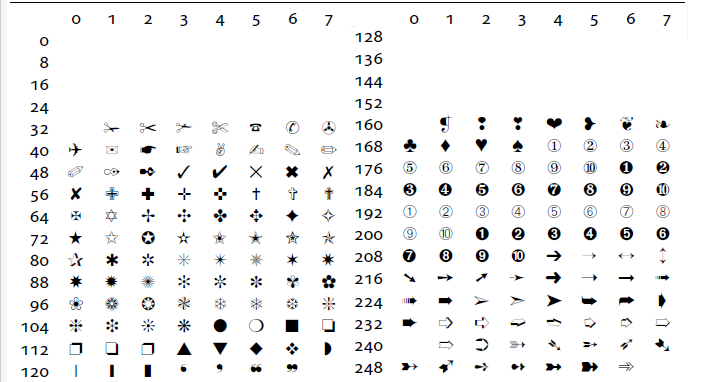
\includegraphics[width=0.9\linewidth]{figure/00123}
\end{figure}
\begin{note}
	凑合看吧,懒得分图了!,有序差不多就是这些内容!基本上够用了。
\end{note}


\subsection{有序列表}
召唤一个有序列表:
\begin{tcblisting}{sidebyside}
\begin{enumerate}
\item 这是有序1
\item 这是有序2
\item 这是有序3
\end{enumerate}
\end{tcblisting}

\begin{note}
	关于有序列表是不是可以自定义序号的样式,答案是肯定有,但是涉及到修改命令了,有点费事,就不说了,空了可以自己去看,这里给出一些简单方法实现。
\end{note}

\begin{tcblisting}{sidebyside}
\begin{enumerate}[(I)]
\item 这是有序1
\item 这是有序2
\item 这是有序3
\end{enumerate}
\end{tcblisting}
\begin{tcblisting}{sidebyside}
\begin{enumerate}[(i)]
\item 这是有序1
\item 这是有序2
\item 这是有序3
\end{enumerate}
\end{tcblisting}
\begin{tcblisting}{sidebyside}
\begin{enumerate}[(A)]
\item 这是有序1
\item 这是有序2
\item 这是有序3
\end{enumerate}
\end{tcblisting}
\begin{tcblisting}{sidebyside}
\begin{enumerate}[(a)]
\item 这是有序1
\item 这是有序2
\item 这是有序3
\end{enumerate}
\end{tcblisting}
\begin{tcblisting}{sidebyside}
\begin{enumerate}[{a}-1]
\item 这是有序1
\item 这是有序2
\item 这是有序3
\end{enumerate}
\end{tcblisting}
\begin{tcblisting}{sidebyside}
\begin{enumerate}[Ex i]
\item 这是有序1
\item 这是有序2
\item 这是有序3
\end{enumerate}
\end{tcblisting}
\begin{note}
	有序的嵌套,其实和无序的嵌套是一样的,,符号也是可以自定义的,可以看看简单的嵌套
\end{note}
\begin{tcblisting}{sidebyside}
\begin{enumerate}
\item 这是有序1
\begin{enumerate}
\item  这是有序1.1
\item  这是有序1.2
\item  这是有序1.3
\end{enumerate}
\item 这是有序2
\begin{enumerate}
\item  这是有序2.1
\item  这是有序2.2
\item  这是有序2.3
\end{enumerate}
\item 这是有序3
\begin{enumerate}
\item  这是有序3.1
\item  这是有序3.2
\item  这是有序3.3
\end{enumerate}
\end{enumerate}
\end{tcblisting}
\begin{note}
	其实我在做这块的时候,更想要的是那种带圈的数字,如何实现的,复杂方法的我们可以通过改命令实现,简单的我们可以掉包实现dingaotolist,注意这里貌似只有172和202才可以用,其他的不行,最大排到10,想更多的话,改命令实现!!!
\end{note}
\begin{tcblisting}{sidebyside}
\begin{dingautolist}{172}
\item  这是有序1
\item  这是有序2
\item  这是有序3
\end{dingautolist}
\end{tcblisting}
\begin{tcblisting}{sidebyside}
\begin{dingautolist}{202}
\item  这是有序1
\item  这是有序2
\item  这是有序3
\end{dingautolist}
\end{tcblisting}
\subsection{解说列表}
不废话这玩意就是对一些专业术语做解释用的,直接看示例:
\begin{tcblisting}{sidebyside}
\begin{description}
\item[词条1] 这是词条的解释语言......
\item[词条2] 这是词条的解释语言......
\item[词条3] 这是词条的解释语言......
\end{description}
\end{tcblisting}
\subsection{通用列表环境list}
\begin{lstlisting}[style=R]
\begin{list}{默认编号}{声明}
	\item [标号] 条目1  
	\item [标号] 条目2
	.......
	\item [标号] 条目?
\end{list}
\end{lstlisting}

\begin{description}
	\item[默认标号] 在条目之前加入的标号,若条目命令\verb|\item|没有给出可选参数标号的话,就使用默认标号了,都不设置,那就都没了
	\item[声明] 针对条目标号,字体,尺寸等样式的设置命令
\end{description}
\begin{note}
	不会高级用法,那就针对每个条目手动编号,没办法技术达不到!看下示例
\end{note}

\begin{tcblisting}{sidebyside}
\begin{list}{}{}
\item [A-I] 这是条目1
\item [A-II] 这是条目2
\end{list}
\end{tcblisting}
\begin{tcblisting}{sidebyside}
\begin{list}{}{}
\item [{\bfseries 步骤1:}] 这是条目1
\item [{\bfseries 步骤2:}] 这是条目2
\end{list}
\end{tcblisting}

\subsection{列表宏包enumitem}
这玩意看看就行,别较真!
\begin{tcblisting}{sidebyside}
\begin{enumerate}[label=\fcolorbox{blue!30}
{cyan!40}{\ding{\value*}},start=172
,itemsep=0pt]
\item 这是步骤1
\item 这是步骤2
\item 这是步骤3
\end{enumerate}
\end{tcblisting}




\chapter{LaTeX 入门之插图篇}
\begin{introduction}
	\item 图形分类
	\item 基本插图
	\item 插图参数
	\item 图片标题与浮动
	\item 多个插图放置
	\item eps图像获取
\end{introduction}
\section{图形的分类}

\subsection{位图图像}
也成为点阵图形,技术上称为栅格图像,它使用称作像素点的小方形组成的网格表示图像,每个像素有自己特定的位置和颜色值。

位图图像可分为无损压缩格式和有损压缩格式。无损压缩格式的有点事能够完整的保存图像的像素信息,但是压缩率比较低。有损压缩技术可以大幅度压缩图形文件,但是会使图形的像素降低。常用的图形文件中TIFF、PNG和GIF都是无损压缩格式,jpg是有损压缩格式。

\subsection{向量图形}

向量图形是由数学公式定义的线段和曲线组成的图形,这些线段和曲线称为向量、改变这些向量的位置、形状、长短和颜色都不会影响图形的品质。向量图形与分辨率无关,也就是说,可以将其任意缩放旋转,按任意分辨率打印都不会失真。因此这是最适合的图形,但是获取难度较大。

\subsection{插图的基本命令}
当需要在源文件插入图片时,首先应当调用$David Carlisle$编写的graphicx宏包。
使用方法如下:
\begin{lstlisting}[style=R]
\usepackage{graphicx} %将该命令放置在导言区
\end{lstlisting}
然后使用插图命令:
\begin{lstlisting}[style=R]
\includegraphics[参数1=选项,参数2=选项,.....]{插图}
\end{lstlisting}
\begin{note}
	插图的参数通常很多,下面我们会介绍常用的一些插图参数!召唤一个图片感受下先。
\end{note}


\begin{tcblisting}{sidebyside}

\includegraphics[width=1\linewidth]{welt.jpg}
\end{tcblisting}
\begin{note}
这里需要注意的是,插图的图片要和你的编译的源文件放在同一目录下,上述\verb|[width=1\linewidth]|这个参数就是说,插图的宽度等于当前文本行的宽度,
\end{note}
下面我们会具体介绍插图的一些参数.
\section{插图命令的参数}
在graphicx宏包中提供的各种与插图有关的命令中最常用的就是插图命令,即就是上面写到的这个命令:
\begin{lstlisting}[style=R]
\includegraphics[参数1=选项,参数2=选项,.....]{插图}
\end{lstlisting}

其中插图是所要插入图形的名称,包括扩展名,下来就是这些参数,大概可被分为三类,\underline{外形参数,裁剪参数,和布尔参数}。其中我们平时写作中用的最多的是外形参数,关于裁剪参数,其中的命令主要用于设置插图的显示区域,一般很少用到,因为在插图时一般会直接将想要插入的图片裁减好才进行插入,当然你想在插入的时候裁剪,你可以自己找下参考书,或者找度娘。关于布尔参数,用的也比较少,一般我们在插图过程中设定的高度或者宽度不成比例的情况下,可能会造成图片失真,这时候通过设置布尔参数中的某些参数,将会按照原图的高宽比例缩放到设定的宽度或高度,但不会超出所设定高度或者宽度。
\begin{note}
关于三种参数,我们必须要掌握的是外形参数,知道这些参数足以解决百分之九十的问题。
\end{note}
\subsection{外形参数说明}
\begin{dinglist}{118}
	\item height: 设定插图的高度,可使用系统认可的长度单位
	\item totalheight: 设置插图的总高度。总高度= 高度+深度。
	\item width:设置插图的宽度。
	\item scale:设置图片的缩放系数,scale=2,表示将图片放大两倍插入,当它是个负值时,则表示在缩放的同时,将插图逆时针旋转$180^{\circ}$
	\item 还有个origin用于设置插图的旋转点,很少用,bb参数用于设定EPS格式图片的BoundingBOX值,一个插图的坐标值。
\end{dinglist}


\subsection{关于图片的高度与深度}
\begin{figure}[H]
	\centering
	\includegraphics[width=0.8\linewidth]{figure/11843}
	\caption{这是图片的高度与深度}
\end{figure}

关于高度和总高度这些我个人一般很少去定义,因为直接这样定义图片可能会变得很难看,通常情况都是通过设置宽度和当前文本行的数值关系去设置,高度这时会自动调整,或者使用缩放这个命令进行调整。具体示例如下:
\begin{tcblisting}{sidebyside}
设置图像宽度是文本宽度的$50\%$:


\includegraphics[width=0.5\linewidth]{welt.jpg}
\end{tcblisting}
\begin{tcblisting}{sidebyside}
设置图像宽度和文本宽度相同:


\includegraphics[width=1\linewidth]{welt.jpg}
\end{tcblisting}
\subsection{设置图片的缩放}
图片的缩放可以这样子去设置。
\begin{tcblisting}{sidebyside}
这里的图片缩放系数为原图的$1/10$:


\includegraphics[scale=0.1]{12101.jpg}
\end{tcblisting}

\begin{tcblisting}{sidebyside}
这里的图片缩放系数为原图的$1/20$:


\includegraphics[scale=0.05]{12101.jpg}
\end{tcblisting}

\begin{note}
关于负值的设置,感觉没必要,可以先设置缩放,然后再设置旋转,直接使用负值进行缩放旋转,图片样式不太好看,这里不做展示,有兴趣可以试试:
\end{note}
\begin{lstlisting}[style=R]


\includegraphics[scale=0.1]{12101.jpg}


\includegraphics[scale=-0.1]{12101.jpg}
\end{lstlisting}
\subsection{关于图片的旋转}
图片的旋转一般情况用的很少,但是偶尔也会使用。
\begin{tcblisting}{sidebyside}
默认不旋转


\includegraphics[width=0.6\linewidth]{121.png}
\end{tcblisting}

\begin{tcblisting}{sidebyside}
旋转$180^\circ$,默认旋转点为1B基准点


\includegraphics[width=1\linewidth,
angle=180]{121.png}
\end{tcblisting}
这里给出旋转中心的参考图,可以根据旋转点的设置,从而实现不同的旋转效果!就不再一一介绍了。
\begin{figure}[H]
	\centering
	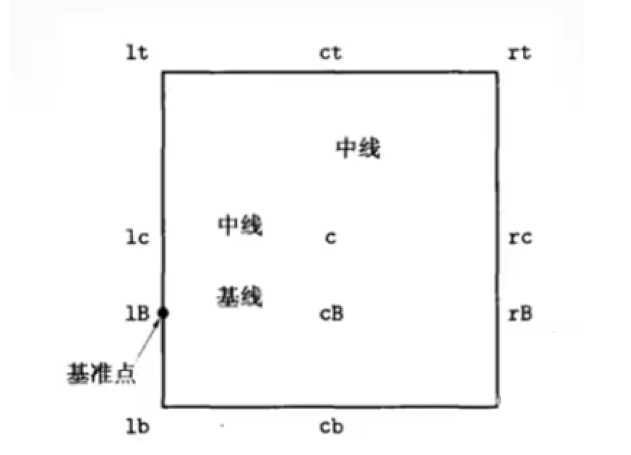
\includegraphics[width=0.8\linewidth]{figure/xzd}
	\caption{旋转中心参考}
\end{figure}

\section{图片的标题和浮动}
在以上内容中我们只是简单的插入一张图片,并未做图片标题和图片位置的设置,这时不合理的,现在我们看下如何设置这些内容,同表格一样,表格有一个table环境用于设置这些信息,图片的话,我们则可以使用figure环境进行设置。示例如下:
\begin{tcblisting}{sidebyside}
\begin{figure}[H]
\centering

\includegraphics[width=0.8\linewidth]
{figure/welt}
\caption{这是薇尔莉特}
\end{figure}
\end{tcblisting}

关于命令的解释如下:

\begin{enumerate}
	\item \verb|\centering|这是用来使图片居中用
	\item \verb|\caption{标题}|这是用来设置标题信息的
	\item \verb|\begin{figure}[H]|这里给出了一个H参数,设置浮动用的
\end{enumerate}
\begin{note}
关于浮动,默认情况是htbp参数,具体可以参照表格浮动部分,这里就不在赘述了。两者基本是一样的
\end{note}

\section{多个插图放置}
这个才是关心的重点!!
\subsection{两图并列,共享标题}
\begin{tcblisting}{sidebyside}
\begin{figure}[H]
\centering

\includegraphics[width=0.45\linewidth]{22.jpg}
 %插入的第一个图片

\includegraphics[width=0.45\linewidth]{22.jpg}
 %插入的第二张图片
\caption{这是日向}
\end{figure}
\end{tcblisting}
貌似这样子有点小了!后面用代码框吧!
\begin{figure}[H]
	\centering
	
\includegraphics[width=0.45\linewidth]{welt1.jpg}
	%插入的第一个图片
	
\includegraphics[width=0.45\linewidth]{welt.jpg}
	%插入的第二张图片
	\caption{紫罗兰永恒花园}
\end{figure}

\begin{lstlisting}[style=R]
\begin{figure}[H]
\centering

\includegraphics[width=0.45\linewidth]{welt1.jpg}
%插入的第一个图片

\includegraphics[width=0.45\linewidth]{welt.jpg}
%插入的第二张图片
\caption{紫罗兰永恒花园}
\end{figure}
\end{lstlisting}
\begin{note}
这里其实容易出问题的是图片大学不一样怎么版,通常我的解决办法是,从一开始就把两图片的大小设置成一样的,或者通过改参数实现。关于参数如何改,多改改就用经验了!O(∩\_∩)O
\end{note}
\begin{figure}[H]
	\centering
	
\includegraphics[width=0.4\linewidth]{welt1.jpg}
	%插入的第一个图片
	
\includegraphics[width=0.53\linewidth]{welt.jpg}
	%插入的第二张图片
	\caption{紫罗兰永恒花园}
\end{figure}

\begin{lstlisting}[style=R]
\begin{figure}[H]
\centering

\includegraphics[width=0.4\linewidth]{welt1.jpg}
%插入的第一个图片

\includegraphics[width=0.53\linewidth]{welt.jpg}
%插入的第二张图片
\caption{紫罗兰永恒花园}
\end{figure}
\end{lstlisting}


\subsection{两图并列,各有标题,共享标题}
\subsubsection{实现方法1}
一图胜千言,直接看效果!
\begin{figure}[H]
	\begin{minipage}{0.5\linewidth}
		\centering
		
\includegraphics[width=0.9\linewidth]{yg.jpg}
		\caption{白骑士$\cdot$月光}
	\end{minipage}	
	\begin{minipage}{0.5\linewidth}
		\centering
		
\includegraphics[width=0.8\linewidth]{12101.jpg}
		\caption{御神装$\cdot$勿忘}
	\end{minipage}	
	\caption{这是崩坏三}
\end{figure}
实现代码:
\begin{lstlisting}[style=R]
\begin{figure}[H]
\begin{minipage}{0.5\linewidth}
\centering

\includegraphics[width=0.9\linewidth]{yg.jpg}
\caption{白骑士$\cdot$月光}
\end{minipage}	
\begin{minipage}{0.5\linewidth}
\centering

\includegraphics[width=0.8\linewidth]{12101.jpg}
\caption{御神装$\cdot$勿忘}
\end{minipage}	
\caption{这是崩坏三}
\end{figure}
\end{lstlisting}
代码解释:

这里使用了一个minipage环境,第一个minipage设置环境的长度等于1/2的线宽,第二个环境也是一样的,然后外面套一个大的figure环境就可以了!

\subsubsection{实现方法2}
\begin{figure}[H]
	\centering
	\subfloat[白骑士$\cdot$月光]{
		
\includegraphics[width=0.48\linewidth]{yg.jpg}}
	\hspace{10pt}
	\subfloat[御神装$\cdot$勿忘]{
		
\includegraphics[width=0.4\linewidth]{12101.jpg}}
	\caption{这是崩坏三}
\end{figure}
实现代码:
\begin{lstlisting}[style=R]
\begin{figure}[H]
\centering
\subfloat[白骑士$\cdot$月光]{

\includegraphics[width=0.48\linewidth]{yg.jpg}}
\hspace{10pt}
\subfloat[御神装$\cdot$勿忘]{

\includegraphics[width=0.4\linewidth]{12101.jpg}}
\caption{这是崩坏三}
\end{figure}
\end{lstlisting}
代码解释:

首先你需要在导言区导入subfig浮动体宏包,然后就是关于它的用法:
\begin{lstlisting}[style=R]
%导言区
\usepackage{subfig}
%正文区
\subfloat[表格标题]]{图形或者表格}
\end{lstlisting}
然后两者嵌套即可,其中\verb|\hspace{10pt}|这是为了设置水平间距用的!

\subsubsection{实现方法3}
还以通过前面学过的表格环境进行实现
\begin{figure}[H]
	\centering
	\begin{tabular}{cc}
		
\includegraphics[width=0.5\linewidth]{yg.jpg} &
		
\includegraphics[width=0.42\linewidth]{12101.jpg} \\
		(白骑士$\cdot$月光) & (御神装$\cdot$勿忘)  \\
	\end{tabular}
	\caption{这是崩坏三}
\end{figure}
代码实现:
\begin{lstlisting}[style=R]
\begin{figure}[H]
\centering
\begin{tabular}{cc}

\includegraphics[width=0.5\linewidth]{yg.jpg} &

\includegraphics[width=0.42\linewidth]{12101.jpg} \\
(白骑士$\cdot$月光) & (御神装$\cdot$勿忘)  \\
\end{tabular}
\caption{这是崩坏三}
\end{figure}
\end{lstlisting}
\subsection{其他插图}
\begin{center}
figure+subfloat
\end{center}

\begin{figure}[H]
	\centering
	\subfloat[pic1]{{\label{pic1}}
		
\includegraphics[width=0.3\linewidth]{1.png}}
	\hspace{10pt}
	\subfloat[pic2]{{\label{pic1}}
		
\includegraphics[width=0.3\linewidth]{2.png}}
	\subfloat[pic3]{{\label{pic1}}
		
\includegraphics[width=0.3\linewidth]{3.png}}
	\caption{这是总标题}
\end{figure}
代码实现:
\begin{lstlisting}[style=R]
\begin{figure}[H]
\centering
\subfloat[pic1]{{\label{pic1}}

\includegraphics[width=0.3\linewidth]{1.png}}
\hspace{10pt}
\subfloat[pic2]{{\label{pic1}}

\includegraphics[width=0.3\linewidth]{2.png}}
\subfloat[pic3]{{\label{pic1}}

\includegraphics[width=0.3\linewidth]{3.png}}
\caption{这是总标题}
\end{figure}
\end{lstlisting}
\begin{center}
figure+tabular
\end{center}

\begin{figure}[H]
\begin{tabular}{cc}
	
\includegraphics[width=0.4\linewidth]{121.png} &
	
\includegraphics[width=0.4\linewidth]{121.png} \\
	(a) & (b) \\
	
\includegraphics[width=0.4\linewidth]{121.png} &
	
\includegraphics[width=0.4\linewidth]{121.png} \\
	(c) & (d) \\
\end{tabular}
\caption{四个日向}
\vspace{-0.5em}
\end{figure}
代码实现
\begin{lstlisting}[style=R]
\begin{figure}[H]
\begin{tabular}{cc}

\includegraphics[width=0.4\linewidth]{121.png} &

\includegraphics[width=0.4\linewidth]{121.png} \\
(a) & (b) \\

\includegraphics[width=0.4\linewidth]{121.png} &
\includegraphics[width=0.4\linewidth]{121.png} \\
(c) & (d) \\
\end{tabular}
\caption{四个日向}
\vspace{-0.5em}
\end{figure}
\end{lstlisting}


\begin{center}
figure+minipage	
\end{center}
\begin{figure}[H]
	\begin{minipage}{0.5\linewidth}
		\centering
		\includegraphics[width=0.9\linewidth]{111.png}
		\caption{这是图一}
	\end{minipage}	
	\begin{minipage}{0.5\linewidth}
		\centering
		\includegraphics[width=0.9\linewidth]{111.png}
		\caption{这是图一}
	\end{minipage}	
	
	\begin{minipage}{0.5\linewidth}
		\centering
		\includegraphics[width=0.9\linewidth]{111.png}
		\caption{这是图三}
	\end{minipage}
	\begin{minipage}{0.5\linewidth}
		\centering
		\includegraphics[width=0.9\linewidth]{111.png}
		\caption{这是图四}
	\end{minipage}
	
	\caption{这是总的标题}
\end{figure}
代码实现
\begin{lstlisting}[style=R]
\begin{figure}[H]
\begin{minipage}{0.5\linewidth}
\centering
\includegraphics[width=0.9\linewidth]{111.png}
\caption{这是图一}
\end{minipage}	
\begin{minipage}{0.5\linewidth}
\centering
\includegraphics[width=0.9\linewidth]{111.png}
\caption{这是图一}
\end{minipage}	

\begin{minipage}{0.5\linewidth}
\centering
\includegraphics[width=0.9\linewidth]{111.png}
\caption{这是图三}
\end{minipage}
\begin{minipage}{0.5\linewidth}
\centering
\includegraphics[width=0.9\linewidth]{111.png}
\caption{这是图四}
\end{minipage}

\caption{这是总的标题}
\end{figure}
\end{lstlisting}
\begin{note}
minipage 是采用行方向累加制的自动排版方法,也就是当子图的width 累计大于
等于\verb|\linewidth|时,后续的图片自动排到下一行,关于这里面的区别,表格应该是最简单好理解的,但是问题是,表格实现的不能进行引用,而使用minipage或者其他实现的可以进行交叉引用,关于交叉引用看吧,空了在参考文献部分讲吧!那玩意不是太难!
\end{note}

\section{eps图像获取}
\begin{lstlisting}[style=R] 
for /f %%i in ('dir /b *.jpg *.jpeg *.bmp *.png') do (
@echo %%i
bmeps -c %%i %%~ni.eps
@echo Finished
)
pause
\end{lstlisting}
\chapter{LaTeX 入门之参考参考文献篇}
\begin{introduction}
	\item 参考文献
	\item 交叉引用
	\item 代码框设计
	\item 网址链接
\end{introduction}
这一部分本来只想写参考文献的,但是还是打算把其他内容补充进去,就是这样子!
\section{参考文献}
这部分主要介绍两种参考文献的使用方式,一种是基本的参考文献和引用。另外一种则是使用bibtex数据库进行参考文献的管理。


\subsection{什么是参考文献}
参考文献是在学术研究过程中,对某一著作或论文的整体的参考或借鉴。征引过的文献在注释中已注明,不再出现于文后参考文献中。

按照字面的意思,参考文献是文章或著作等写作过程中参考过的文献。然而,按照GB/T 7714-2015《信息与文献 参考文献著录规则》”的定义,文后参考文献是指:“为撰写或编辑论文和著作而引用的有关文献信息资源。根据《中国学术期刊(光盘版)检索与评价数据规范(试行)》和《中国高等学校社会科学学报编排规范(修订版)》的要求,很多刊物对参考文献和注释作出区分,将注释规定为“对正文中某一内容作进一步解释或补充说明的文字”,列于文末并与参考文献分列或置于当页脚地。


\subsection{基本的参考文献}
首先我们召唤一波参考文献!
\begin{lstlisting}[style=R]
刘国钧,陈绍业,王凤翥. 图书馆目录[M]. 北京:高等教育出版社,1957.15-18.

辛希孟. 信息技术和信息服务国际研讨会论文集:A集[C]. 北京:中国社会科学出版社,1994.

张筑生. 微分半动力系统的不变集[D]. 北京:北京大学数学系数学研究所,1983.

冯西桥. 核反应堆压力管道和压力容器的LBB分析[R]. 北京:清华大学核能技术设计研究院,1997.
\end{lstlisting}
这是随便找的一些参考文献,两步问题,首先这玩意怎么插到文章,然后如何引用这些参考文献。关于参考文献的书写格式,因为各个期刊要求的都不太相同,所以没办法统一介绍,这部分就需要你参照你写文章的期刊是怎么要求了。

现在我们先看下参考文献的环境是什么样的。如下代码所示:
\begin{lstlisting}[style=R]
\begin{thebibliography}{最大序号}
\bibitem[文献序号1]{检索名} 文献信息
\bibitem[文献序号2]{检索名} 文献信息
\bibitem[文献序号3]{检索名} 文献信息
.......
\end{thebibliography}
\end{lstlisting}
参数说明如下:
\begin{enumerate}
	\item 最大序号:用于测定文献列表中文献序号的最大宽度,如果你是10以内的参考文献,那就用9,超过10小于100那就填99.
	\item 文献序号:可选参数,用于设定该条文献在参考文献列表中的序号。
	\item 检索名:为该文献信息起的简短名称,
	\item 文献信息:就是参考文献内容了。
\end{enumerate}
这就是参考文献的书写了,然后就是关于参考文献的引用。
\subsection{参考文献的引用}
如果要在正文中引用参考文献列表中的文献时,可以在引文之后插入文献的引用命令:
\begin{lstlisting}[style=R]
\cite[附加信息]{检索名1,检索名2....}
\end{lstlisting}
参数说明如下:
\begin{enumerate}
	\item 检索名:就是文献条目中的\verb|\bibitem|中的检索名,引用那条文献,就指定那条文献的检索名,可以指定多个检索名,中间使用逗号分割(半角逗号)且不留空格。
	\item 附加信息:可选参数,可以用作对所引用参考文献的注解。例如文献过长,可以使用附加信息说明参考内容的页码范围。
\end{enumerate}
\subsection{引文格式修改}
还是比较有用的吧!在引用的标志中如果有多个参考文献序号,可能会出现[4,6,5]这种跳号情况,文献序号之间间隔无法调整,这时候可以调用cite宏包进行修改。使用命令如下:
\begin{lstlisting}[style=R]
\usepackage[格式]{cite}
\end{lstlisting}
命令说明,可以通过修改格式这个可选参数来对引用格式进行修改,常见参数如下:
\begin{enumerate}
	\item biblable:将参考文献的列表中的文献序号改成上标形式
	\item noadjust:不在引文与\verb|\cite|中插入一个空格,默认是adjust,会插入一个空格。
	\item nocompress:不将引用标志中三个以上的连续序号改为范围序号,差不多是这样,如果你默认是$[4,5,6]$那么系统默认会给你改成$[4-6]$
	\item nosort:不对引用标志的序号进行排序,默认是排的。
	\item nospace:取消分隔逗号的空格。默认是有的。
	\item ref:在序号前加入参考文献缩写:Ref.。
	\item super:取消引用标志,将其中的序号改用上标格式显示,这是引用命令中不能出现附加信息的可选参数,否则仍按默认选项
\end{enumerate}

或者使用natbib宏包,看起来这个更好用些,natbib 重新实现了 \verb|\cite| 命令以适应作者--年和编号两种形式的引用,完全兼容标准的文献样式 plain, alpha, unsrt等,也可以配合 harvard, apalike, chicago, astron, authordate 等样式要求。
\begin{lstlisting}[style=R]
\usepackage[option]{natbib}
\end{lstlisting}
option参数说明:
\begin{enumerate}
	\item round: (default) 使用圆括号
	\item square: 使用方括号
	\item curly: 使用花括号
	\item angle: 使用尖括号
	\item colon: (default) 用引号分隔多个引用
	\item comma: 用逗号分隔多个引用
	\item authoryear: (default) 使用作者--年引用形式
	\item numbers: 使用编号引用形式
	\item super: 使用 Nature 那样的上标编号引用
	\item sort: 多个引用按照首字母排序
	\item sort\&compress: 除排序外,多个引用可以合并 (如 3-6, 15)
	\item longnamesfirst: 多个作者的文献第一次被引用时列出所有作者,以后的引用可以缩写为 et al.
\end{enumerate}
注意有的文档在一开始就给你把参考文献的样式做过限定,比如这个模板,那么如何去更改呢?在导言区重定义下你的命令就可以了,解释涉及到命令修改,算了!

\verb|\newcommand{\upcite}[1]{$^{\mbox{\scriptsize \cite{#1}}}$}|

\subsection{bibtex文献管理使用}
使用方式:
\begin{lstlisting}[style=R]
\bibliographystyle{文献格式名}
\bibliography{文献数据库名}
\end{lstlisting}
\begin{itemize}
	\item 文献格式名,这个一般有所选的参考期刊给定,常用的plain,unsrt,alpha,abbrv,ieetr等等。
	\item 文献数据库,BibTeX的bib文件是一个记录已阅文献的数据库,但是通常不建议手动编译bib文件,
\end{itemize}
建议:
\begin{enumerate}
	\item 使用JabRef或Zotero等文献管理工具导出bib文件创
	\item 使用Google Scholar或Bing学术导出bib条目建
\end{enumerate}
引文的信息还有很多国内外网站可以获取包括:
百度学术、搜狗学术,万方、维普......很多,

有时候参考文献出现问题,需要重构怎么办?使用notepad++等一些字处理软件进行更改,但是不建议自己手动写bib文件。
\section{交叉引用}
使用/lable{标号}来定义标号, 这里的标号可以是字母,
数字, 标点等组成的字符串. 需要引用, 则使用/ref{标号}, 这
里的"标号"应该是有/lable定义过的, 定义和引用的先后无关.

\section{网址链接}
调用宏包:
\begin{lstlisting}[style=R]
\usepackage{hyperef}
\end{lstlisting}


\begin{lstlisting}[style=R]
\href{}{文字} 命令可以用来使文字产生指向URL地址的超链接效果。
\end{lstlisting}

\section{代码框设计}
\begin{lstlisting}[style=R]

\usepackage{listings}%插入代码

\lstset{numbers=left, %设置行号位置

numberstyle=\tiny, %设置行号大小

keywordstyle=\color{blue}, %设置关键字颜色

commentstyle=\color[cmyk]{1,0,1,0}, %设置注释颜色

frame=single, %设置边框格式

escapeinside=``, %逃逸字符(1左面的键),用于显示中文

%breaklines, %自动折行

extendedchars=false, %解决代码跨页时,章节标题,页眉等汉字不显示的问题

xleftmargin=0em,xrightmargin=0em, aboveskip=1em, %设置边距

tabsize=4, %设置tab空格数

%showspaces=false %不显示空格

breaklines,%自动换行

columns=flexible,%不随便添加空格,只在已经有空格的地方添加空格,

%如果想要添加空格使用fixed作为参数(这是默认的),如果坚决不添加空格使用fullflexible作为参数

\end{lstlisting}
这部分还有很多!


\end{document}
